%Version 3 October 2023 (Springer Nature LaTeX template, sn-jnl)
\documentclass[pdflatex,sn-mathphys-num]{sn-jnl}% Math and Physical Sciences Numbered Reference Style

%%%% Standard packages from the template
\usepackage{graphicx}%
\usepackage{multirow}%
\usepackage{amsmath,amssymb,amsfonts}%
\usepackage{amsthm}%
\usepackage{mathrsfs}%
\usepackage[title]{appendix}%
\usepackage{xcolor}%
\usepackage{textcomp}%
\usepackage{manyfoot}%
\usepackage{booktabs}%
\usepackage{algorithm}%
\usepackage{algorithmicx}%
\usepackage{algpseudocode}%
\usepackage{listings}%
%%%% Additional packages for this paper
\usepackage{tikz}%
\usetikzlibrary{positioning,arrows.meta,calc,fit,backgrounds}%
\usepackage{tabularx}%

\lstset{basicstyle=\ttfamily\footnotesize,columns=fullflexible,keepspaces=true,
  breaklines=true,frame=single,framerule=0.3pt,xleftmargin=2pt,xrightmargin=2pt,
  aboveskip=6pt,belowskip=6pt}
\renewcommand{\lstlistingname}{Listing}

\newcolumntype{L}[1]{>{\raggedright\arraybackslash}p{#1}}%
\newcolumntype{Y}{>{\raggedright\arraybackslash}X}%

\raggedbottom

\begin{document}

\title[Where Does Virtual Machine Boot Time Go?]{Where Does Virtual Machine Boot Time Go? A Controlled Comparison of MicroVMs, a Traditional VM and a Container on KVM}

\author*[1]{\fnm{Sanyam} \sur{Budwal}}\email{sanyam.budwal.ug24@nsut.ac.in}

\author[1]{\fnm{Aashi} \sur{Bhatt}}\email{aashi.bhatt.ug24@nsut.ac.in}

\author[1]{\sur{Sohaib}}\email{mohammad.sohaib.ug24@nsut.ac.in}

\affil*[1]{\orgdiv{Department of Information Technology}, \orgname{Netaji Subhas University of Technology}, \orgaddress{\city{New Delhi}, \country{India}}}

\abstract{Serverless and multi-tenant cloud platforms need isolated execution environments that start in milliseconds, which has driven the adoption of minimal virtual machines (microVMs) such as AWS Firecracker. Published comparisons usually report how long each platform takes to start, but rarely separate the time spent by the guest operating system from the time spent by the virtual machine monitor (VMM) that hosts it. We present a controlled, reproducible study on a single commodity desktop running KVM. We compare a traditional VM (QEMU \texttt{q35} with firmware, a bootloader and a full Fedora system), QEMU's \texttt{microvm} machine type, Firecracker, and a Podman container. Both microVMs boot an identical kernel and root filesystem, and we combine host wall-clock measurements with timestamps from the guest kernel log to split each boot into guest time and VMM time. A tuned Firecracker microVM completed a full boot-and-shutdown cycle in 118.6\,ms on average (30 runs), about 106 times faster than the traditional VM reached a booted state (12.55\,s) and slightly faster than a Podman container start (135.4\,ms). The guest kernel took a similar time on both microVMs (42.5\,ms and 49.1\,ms), while the remaining VMM-side time fell from 120.0\,ms with QEMU to 69.5\,ms with Firecracker, a 42\% reduction. Out of the box, however, Firecracker was 5.3 times slower than after tuning, because the guest probed an emulated keyboard controller for about 0.48\,s. Printing boot messages to the emulated serial console more than doubled boot time on both VMMs. With 20 identical VMs, Kernel Samepage Merging (KSM) reduced QEMU microVM memory from 70.0 to 44.2\,MiB per VM, while Firecracker, which does not mark guest memory as mergeable, used 44.9\,MiB per VM without any deduplication. These results show that VM startup cost is dominated by the virtual machine model and the software stack around the guest rather than by hardware virtualization itself.}

\keywords{Virtualization, KVM, MicroVM, Firecracker, QEMU, Serverless computing, Cold start, Memory deduplication}

\maketitle

%% =====================================================================
\section{Introduction}\label{sec:intro}

Cloud platforms run code from many customers on shared physical servers. Each workload must be isolated from the others, and in serverless or Function-as-a-Service (FaaS) platforms the isolated environment must also be created quickly, often for every new burst of requests~\cite{jonas2019berkeley}. The delay between a request arriving and an environment being ready to serve it is known as a \emph{cold start}. A characterisation of the production Azure Functions workload showed that cold starts are frequent enough to matter for both latency and provider cost~\cite{shahrad2020wild}, and two recent surveys catalogue a large body of work on reducing them~\cite{golec2024coldstart,ghorbian2024survey}.

Two isolation technologies dominate. \emph{Containers} run workloads as fenced-off groups of processes on the host's own kernel. They start quickly and use little memory, but every container shares one kernel, so a kernel vulnerability can expose all of them. \emph{Virtual machines} (VMs) give each workload its own kernel and use hardware virtualization to enforce the boundary, which is stronger, but a conventional VM imitates a complete PC and boots a general-purpose operating system, which takes seconds. \emph{MicroVMs} try to combine the two. Firecracker, which AWS built for Lambda and Fargate, removes the BIOS, the PCI bus and almost every emulated device, and reports guest boot times in the low hundreds of milliseconds~\cite{agache2020firecracker}. QEMU, the most widely used open-source VMM~\cite{bellard2005qemu}, offers a comparable minimal machine type called \texttt{microvm}~\cite{qemumicrovm}.

A boot time measured from outside a VM is a sum of very different costs: starting the VMM process, building the virtual machine, running firmware and a bootloader if they exist, booting the guest kernel, running the guest's first program, and shutting down. When two platforms differ in total time, it is usually unclear which of these parts is responsible. This matters in practice. If the guest kernel dominates, engineers should tune the kernel; if the VMM dominates, they should choose or tune the VMM; if the virtual hardware dominates, they should change the machine model.

This paper asks a single research question: \emph{how much of a VM's startup time and memory comes from the guest operating system, and how much from the virtual machine model and the VMM that presents it?} We test three hypotheses:
\begin{itemize}
\item[\textbf{H1}] MicroVMs boot at least ten times faster than a traditional VM on the same hypervisor.
\item[\textbf{H2}] Most of that difference comes from the virtual machine model and the VMM (firmware, emulated devices, process start-up), not from KVM itself.
\item[\textbf{H3}] Memory deduplication with Kernel Samepage Merging (KSM) lets many identical VMs share memory, at a measurable CPU cost and with known security implications.
\end{itemize}

Our study makes the following contributions:
\begin{enumerate}
\item A controlled comparison of four isolation tiers on one KVM host, in which the two microVMs boot the \emph{same} kernel file and the \emph{same} root filesystem image with the same CPU and memory configuration, so that their differences can only come from the VMM and its virtual hardware.
\item A two-clock decomposition of boot time that combines host wall-clock measurements with the guest kernel's own log timestamps, separating guest kernel time from VMM-side time without modifying either VMM.
\item Three configuration findings, each diagnosed from kernel logs and removed with a one-line change: a kernel panic caused by legacy timer hardware in QEMU's \texttt{microvm}, a 0.48\,s keyboard-controller probe that makes default Firecracker 5.3 times slower than a tuned configuration, and the cost of a verbose serial console.
\item A density experiment with 20 concurrent microVMs that quantifies what KSM saves for QEMU, and shows that Firecracker reaches the same per-VM memory without deduplication.
\item A public repository containing every script, raw log and figure needed to reproduce the study.
\end{enumerate}

The rest of the paper is organised as follows. Section~\ref{sec:background} explains the concepts the study relies on. Section~\ref{sec:related} reviews related work. Section~\ref{sec:method} describes the methodology and system architecture, and Section~\ref{sec:impl} the implementation and experimental setup. Section~\ref{sec:results} presents the results, Section~\ref{sec:discussion} discusses them and their limitations, and Section~\ref{sec:conclusion} concludes.

%% =====================================================================
\section{Background}\label{sec:background}

\subsection{Hypervisors and virtual machine monitors}

Popek and Goldberg defined the conditions under which an instruction set can be virtualized efficiently~\cite{popek1974}. Early x86 processors did not meet them, which led to binary translation and paravirtualization approaches such as Xen~\cite{barham2003xen}. Modern x86 processors add hardware support, Intel VT-x and AMD-V, that lets guest code run directly on the CPU while the processor traps sensitive operations~\cite{uhlig2005vt}.

On Linux this support is exposed by \emph{KVM}, a kernel module that turns the Linux kernel into a hypervisor~\cite{kivity2007kvm}. KVM virtualizes the CPU and memory, but it does not emulate devices, load guest kernels or decide what hardware a VM has. Those tasks belong to a user-space \emph{virtual machine monitor} (VMM), an ordinary process that opens \texttt{/dev/kvm}, allocates guest memory, creates virtual CPUs and emulates devices. QEMU and Firecracker are both VMMs that run on KVM. When a guest accesses an emulated device, for example by writing a character to a serial port, the processor stops running the guest and control passes through KVM to the VMM, which emulates the access and resumes the guest. This round trip is called a \emph{VM exit}. Devices that the guest uses often, or that require many exits, are therefore expensive.

QEMU emulates a wide range of hardware and can run almost any operating system. Its \texttt{q35} machine type imitates a modern PC with a PCI Express bus, booted through SeaBIOS firmware. Its \texttt{microvm} machine type has no PCI bus and no firmware: the VMM loads the kernel directly into guest memory, and devices are attached through the lightweight virtio-mmio transport~\cite{qemumicrovm,russell2008virtio}. Firecracker follows the same direct-boot approach but is a separate, much smaller program written in Rust, emulating only virtio network and block devices, a serial console, a minimal keyboard controller and a few platform devices~\cite{agache2020firecracker}.

\subsection{Containers}

A container is a group of processes isolated with Linux namespaces and resource-limited with control groups. It has no guest kernel to boot, so starting one is a matter of preparing the namespaces and launching a process. Container engines such as Podman add their own management steps, including a small monitor process, \texttt{conmon}, that supervises each container. Containers are cheap because they share the host kernel; for the same reason they offer weaker isolation than VMs~\cite{manco2017lightvm,young2019gvisor}.

\subsection{Copy-on-write disk images}

The \texttt{qcow2} disk format supports \emph{backing files}: a new image can be created as a thin overlay on top of a read-only base image. Reads of unchanged blocks are served from the base, and writes go only to the overlay. Cloud providers use this copy-on-write layering to start many VMs from one shared base image without copying it.

\subsection{Kernel Samepage Merging}

KSM is a Linux feature that scans memory regions that a process has marked as mergeable, finds pages with identical contents, and replaces them with a single write-protected copy~\cite{arcangeli2009ksm,kernelksm}. If any user later writes to a merged page, the kernel transparently gives it a private copy. KSM increases VM density, but it costs CPU time for scanning, and shared pages open timing and Rowhammer-based attacks between the VMs that share them~\cite{suzaki2011dedup,razavi2016ffs}.

%% =====================================================================
\section{Related Work}\label{sec:related}

\subsection{Virtual machines versus containers}

Felter et al.~\cite{felter2015} compared KVM VMs with Docker containers on CPU, memory, storage and network workloads and found that containers matched or exceeded VMs in almost every case, with the largest VM overheads in I/O. Their study concerned steady-state performance rather than start-up. Manco et al.~\cite{manco2017lightvm} argued that VMs can be as light as containers if both the guest and the toolstack are minimised. Using unikernels and a stripped-down Linux on a redesigned Xen toolstack, they reported VM creation times in the millisecond range and densities of thousands of VMs per host, and showed that the toolstack, not the hypervisor, was the main bottleneck. Our results reach a similar conclusion on KVM with unmodified, widely used VMMs. Li et al.~\cite{li2021lightweight} compared Docker, gVisor, Kata Containers on QEMU and on Firecracker, and plain QEMU/KVM, reporting that a QEMU/KVM VM took about 8.76\,s to start while the container-based options started far faster, and that memory use grew from Docker to gVisor to Kata to QEMU/KVM. They treat each platform as a black box; we add a same-guest control and a guest/VMM split.

\subsection{Lightweight virtualization}

Unikernels compile an application and a minimal library operating system into a single image~\cite{madhavapeddy2013unikernels}, and Unikraft makes building them practical~\cite{kuenzer2021unikraft}. They achieve very fast boots but require changing how applications are built. gVisor takes a different path, intercepting system calls in a user-space kernel, and its performance costs were analysed by Young et al.~\cite{young2019gvisor}. Firecracker keeps an unmodified Linux guest and instead minimises the VMM~\cite{agache2020firecracker}. Its authors measured boot time from the VMM process fork until the guest started init, with VMMs modified to exit on a write to a designated I/O port, and found Firecracker and Cloud Hypervisor considerably faster than QEMU, with QEMU about twice as slow. They also reported a VMM memory overhead of about 3\,MB for Firecracker against about 131\,MB for QEMU. Anjali et al.~\cite{anjali2020blending} examined how much host kernel code Firecracker, gVisor and Linux containers exercise and found that both sandboxes still execute substantially more kernel code than native Linux. Kata Containers runs each container inside its own lightweight VM to combine container tooling with VM isolation~\cite{katacontainers}.

\subsection{Serverless cold starts}

Wang et al.~\cite{wang2018peeking} measured cold-start latency and performance isolation across commercial serverless platforms. Shahrad et al.~\cite{shahrad2020wild} characterised the Azure Functions workload and proposed adaptive keep-alive policies to reduce cold starts. Several systems attack the cold start directly: SOCK uses optimised containers and package caching~\cite{oakes2018sock}, Catalyzer restores pre-initialised state to start sandboxes in sub-millisecond time~\cite{du2020catalyzer}, and REAP records and prefetches the working set of Firecracker snapshots~\cite{ustiugov2021reap}. FaaSnap improves snapshot-based VM restore further with per-region memory mapping and concurrent paging~\cite{ao2022faasnap}. More recently, Brooker et al.~\cite{brooker2023ondemand} described how AWS Lambda loads large container images on demand using block-level caching and deduplication, and Sabre uses hardware compression accelerators to shrink Firecracker microVM snapshots and speed up their restore~\cite{lazarev2024sabre}. Golec et al.~\cite{golec2024coldstart} and Ghorbian and Ghobaei-Arani~\cite{ghorbian2024survey} survey this landscape and classify cold-start mitigation techniques.

\subsection{Memory deduplication and its risks}

KSM was introduced to increase the number of VMs a host can run~\cite{arcangeli2009ksm}. Suzaki et al.~\cite{suzaki2011dedup} showed that deduplication creates a timing side channel through which one VM can detect files or applications loaded in another. Razavi et al.~\cite{razavi2016ffs} combined deduplication with Rowhammer to flip bits in a co-located VM's memory. The Firecracker paper accordingly lists disabling samepage merging among its recommended side-channel mitigations~\cite{agache2020firecracker}.

\subsection{Position of this work}

Table~\ref{tab:related} summarises how the studies closest to ours differ. Most snapshot and cold-start systems optimise one platform; most comparisons measure total start-up time per platform. Our study is smaller in scale than industrial evaluations, but it holds the guest constant across two VMMs, splits boot time into guest and VMM components without modifying the VMMs, places a traditional VM and a container in the same harness, and connects start-up time with memory density and deduplication.

\begin{table}[ht]
\caption{Studies closest to this work}\label{tab:related}
\footnotesize
\begin{tabularx}{\textwidth}{@{}L{2.3cm}L{3.6cm}Y@{}}
\toprule
Study & Platforms compared & Focus and method \\
\midrule
Felter et al.~\cite{felter2015} & KVM VM, Docker & Steady-state CPU, memory, storage and network performance \\
Manco et al.~\cite{manco2017lightvm} & Xen with unikernels and Tinyx, Docker & VM creation time and density with a redesigned toolstack \\
Agache et al.~\cite{agache2020firecracker} & Firecracker, Cloud Hypervisor, QEMU & Boot to init with VMMs modified to exit on an I/O write; VMM memory overhead; I/O \\
Anjali et al.~\cite{anjali2020blending} & Firecracker, gVisor, LXC & Host kernel code exercised by each sandbox \\
Li et al.~\cite{li2021lightweight} & Docker, gVisor, Kata (QEMU, Firecracker), QEMU/KVM & Start-up time, memory and performance per platform \\
This work & QEMU \texttt{q35}, QEMU \texttt{microvm}, Firecracker (default and tuned), Podman & Same-guest control, guest/VMM split from two clocks, configuration effects, density with KSM \\
\botrule
\end{tabularx}
\end{table}

%% =====================================================================
\section{Methodology and System Architecture}\label{sec:method}

\subsection{Isolation tiers}

We compare four tiers, summarised in Table~\ref{tab:tiers} and shown in Fig.~\ref{fig:arch}. All three VM tiers run on the same KVM module, so the hypervisor is held constant and only the VMM, the machine model and the guest vary.

\begin{table}[ht]
\caption{Configuration of the four tiers}\label{tab:tiers}
\footnotesize
\begin{tabularx}{\textwidth}{@{}lL{2.0cm}L{3.1cm}YL{1.6cm}@{}}
\toprule
Tier & VMM / runtime & Machine model & Guest & Resources \\
\midrule
T1 & QEMU 10.2.2 & \texttt{q35}, SeaBIOS, GRUB, initrd & Fedora 44 Cloud image, systemd & 1 vCPU, 1024\,MiB \\
T2 & QEMU 10.2.2 & \texttt{microvm}, \texttt{pit=off}, \texttt{pic=off}, direct kernel boot & Linux 6.1.155 + Alpine 3.24.3 rootfs & 1 vCPU, 128\,MiB \\
T3 & Firecracker 1.17.0 & Firecracker default, direct kernel boot & Same kernel and rootfs as T2 & 1 vCPU, 128\,MiB \\
T4 & Podman & None (host kernel shared) & Alpine container & n/a \\
\botrule
\end{tabularx}
\end{table}

\begin{figure}[ht]
\centering
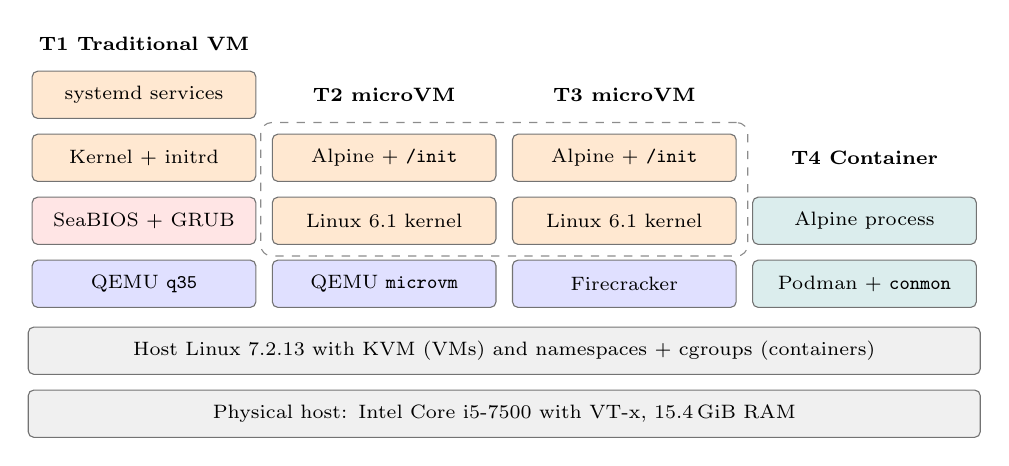
\begin{tikzpicture}[
  font=\scriptsize,
  box/.style={draw=black!55,rounded corners=2pt,text width=2.7cm,minimum height=0.6cm,align=center,inner sep=2pt},
  guest/.style={box,fill=orange!18},
  vmm/.style={box,fill=blue!12},
  host/.style={draw=black!55,rounded corners=2pt,fill=black!6,text width=11.95cm,minimum height=0.6cm,align=center,inner sep=2pt},
  ctr/.style={box,fill=teal!14},
  hd/.style={font=\scriptsize\bfseries,align=center}]
\def\xa{1.45}\def\xb{4.5}\def\xc{7.55}\def\xd{10.6}
\node[host] (hw) at (6.025,0) {Physical host: Intel Core i5-7500 with VT-x, 15.4\,GiB RAM};
\node[host] (kvm) at (6.025,0.8) {Host Linux 7.2.13 with KVM (VMs) and namespaces + cgroups (containers)};
\node[vmm] at (\xa,1.65) {QEMU \texttt{q35}};
\node[vmm] at (\xb,1.65) {QEMU \texttt{microvm}};
\node[vmm] at (\xc,1.65) {Firecracker};
\node[ctr] at (\xd,1.65) {Podman + \texttt{conmon}};
\node[box,fill=red!10] at (\xa,2.45) {SeaBIOS + GRUB};
\node[guest] at (\xa,3.25) {Kernel + initrd};
\node[guest] at (\xa,4.05) {systemd services};
\node[guest] (k2) at (\xb,2.45) {Linux 6.1 kernel};
\node[guest] (u2) at (\xb,3.25) {Alpine + \texttt{/init}};
\node[guest] (k3) at (\xc,2.45) {Linux 6.1 kernel};
\node[guest] (u3) at (\xc,3.25) {Alpine + \texttt{/init}};
\node[ctr] at (\xd,2.45) {Alpine process};
\node[hd] at (\xa,4.7) {T1 Traditional VM};
\node[hd] at (\xb,4.05) {T2 microVM};
\node[hd] at (\xc,4.05) {T3 microVM};
\node[hd] at (\xd,3.25) {T4 Container};
\begin{scope}[on background layer]
\node[draw=black!45,dashed,rounded corners,fit=(k2)(u2)(k3)(u3),inner sep=4pt,
  ] {};
\end{scope}
\end{tikzpicture}
\caption{Architecture of the experiment. All VM tiers share one host kernel and KVM; each VM is created by a user-space VMM. T2 and T3 (dashed box) boot the identical kernel file and root filesystem image. Orange boxes are guest software that a VM must boot and a container does not.}\label{fig:arch}
\end{figure}

T1 represents a conventional VM as commonly deployed: an emulated PC with a PCI bus, firmware, a bootloader, an initial RAM disk (initrd) and a general-purpose distribution managed by systemd. T2 and T3 are microVMs. They boot the same uncompressed Linux 6.1 kernel image, published by the Firecracker project for its continuous-integration tests, and the same 64\,MiB ext4 root filesystem built from the Alpine Linux mini root filesystem. The Alpine userspace is provided by BusyBox and is only a few megabytes. T4, a Podman container, is included as a reference point because microVMs are commonly compared with containers.

Firecracker is measured in two configurations. \emph{T3 default} uses the boot arguments recommended in the project's getting-started material. \emph{T3 tuned} adds four kernel parameters (\texttt{i8042.noaux i8042.nomux i8042.nopnp i8042.dumbkbd}) that stop the guest from probing the emulated keyboard controller (Section~\ref{sec:i8042}). We report both, because the default configuration is what a new user experiences.

\subsection{The guest program}

The microVM guests run the nine-line init script in Listing~\ref{lst:init} as their first and only program. It mounts the \texttt{proc} and \texttt{sysfs} pseudo-filesystems, prints a \texttt{BOOTED} marker, optionally prints the kernel log or sleeps depending on a \texttt{mode=} option on the kernel command line, and then forces an immediate reboot. Both VMMs are configured to exit when the guest resets, so one complete boot corresponds to one host command that can be timed. Because the same script and disk are used for every microVM experiment, the \texttt{mode} option lets one image serve the boot-time, boot-breakdown and memory experiments.

\begin{lstlisting}[caption={Init script of the microVM guest (\texttt{guest/init})},label={lst:init},float=ht]
#!/bin/sh
mount -t proc proc /proc
mount -t sysfs sys /sys
echo "BOOTED guest_uptime=$(cut -d' ' -f1 /proc/uptime)s"
case "$(cat /proc/cmdline)" in
  *mode=dmesg*) dmesg ;;
  *mode=sleep*) sleep 300 ;;
esac
reboot -f
\end{lstlisting}

For T1 we add a small systemd unit to the image. It waits until systemd reports that start-up has finished (\texttt{systemctl is-system-running --wait}), prints \texttt{BOOTED} together with the output of \texttt{systemd-analyze}, and powers the VM off.

\subsection{Two-clock decomposition of boot time}

We measure boot time with two clocks. The \emph{host clock} measures the wall-clock time $T_{\mathrm{wall}}$ of the command that starts the VMM, from process creation until the VMM exits after the guest resets. The \emph{guest clock} is the timestamp that the guest kernel attaches to each line of its log. The kernel prints the line \texttt{Run /init as init process} immediately before it starts the init program, and we use that line's timestamp as the guest kernel boot time $T_{\mathrm{guest}}$.

Because the guest is identical in T2 and T3, the remainder
\begin{equation}
T_{\mathrm{VMM}} = T_{\mathrm{wall}} - T_{\mathrm{guest}}
\label{eq:vmm}
\end{equation}
captures everything that is not guest kernel boot: starting the VMM process, creating the VM and loading the kernel image into guest memory, running the init script, the guest reset, and the VMM's own shutdown. The init script and the reset are identical in both microVMs and take only a few milliseconds, so the difference in $T_{\mathrm{VMM}}$ between T2 and T3 is attributable to the VMMs. We express that difference as a relative reduction
\begin{equation}
R = \frac{T_{\mathrm{VMM}}^{\mathrm{QEMU}} - T_{\mathrm{VMM}}^{\mathrm{FC}}}{T_{\mathrm{VMM}}^{\mathrm{QEMU}}}.
\label{eq:red}
\end{equation}

We deliberately do not use \texttt{/proc/uptime} inside the guest for $T_{\mathrm{guest}}$. In a first verbose QEMU \texttt{microvm} boot, the init script reported \texttt{guest\_uptime=0.17s}, whereas the kernel log placed \texttt{Run /init} at 0.282\,s. The uptime counter starts only once the kernel's timekeeping is initialised, part-way through boot, so it under-reports early boot time. Kernel log timestamps begin much earlier and are used throughout.

For T1, the guest's \texttt{systemd-analyze} reports kernel, initrd and userspace phases. It cannot see the time before the kernel starts on a BIOS system, so we estimate the pre-kernel phase (QEMU start-up, SeaBIOS and GRUB) as the host-measured time until \texttt{BOOTED} minus the total reported by \texttt{systemd-analyze}.

\subsection{Benchmarks}

We run four benchmarks.
\begin{description}
\item[B1, boot latency.] Wall-clock time of a full boot for every tier, using hyperfine~\cite{hyperfine}, which runs a command several times to warm caches and then repeats it and reports the mean, standard deviation and range. A second B1 run measures each microVM with and without the \texttt{quiet} kernel option, to quantify the cost of the serial console.
\item[B2, guest/VMM split.] The guest kernel's \texttt{Run /init} timestamp for T2 and T3, combined with B1 through Eq.~\eqref{eq:vmm}.
\item[B3, single-instance overhead.] Host memory and threads used by one running instance of each tier, plus the size and library dependencies of each VMM binary.
\item[B4, density and KSM.] Memory used by 20 identical concurrent microVMs, before and after enabling KSM.
\end{description}

Algorithm~\ref{alg:boot} summarises B1 and B2, and Algorithm~\ref{alg:ksm} summarises B4.

\begin{algorithm}[ht]
\caption{Boot latency and guest/VMM decomposition (B1, B2)}\label{alg:boot}
\begin{algorithmic}[1]
\Require tiers $\mathcal{T}$, warm-up count $w=3$, runs $n=30$, guest runs $m=10$
\For{each tier $t \in \mathcal{T}$}
  \For{$i \gets 1$ to $w$} \State run $\mathrm{launch}(t,\texttt{quiet})$ \Comment{discarded}
  \EndFor
  \For{$i \gets 1$ to $n$}
    \State $s \gets$ host clock; run $\mathrm{launch}(t,\texttt{quiet})$ until the VMM exits
    \State $T_{\mathrm{wall}}[t,i] \gets$ host clock $- s$
  \EndFor
  \State report mean, standard deviation, minimum and maximum of $T_{\mathrm{wall}}[t,\cdot]$
\EndFor
\For{$i \gets 1$ to $m$} \Comment{T2 and T3 interleaved}
  \For{$t \in \{\mathrm{T2},\mathrm{T3\ tuned}\}$}
    \State $\ell \gets$ console output of $\mathrm{launch}(t,\texttt{quiet mode=dmesg})$
    \State $T_{\mathrm{guest}}[t,i] \gets$ timestamp of line ``\texttt{Run /init as init process}'' in $\ell$
  \EndFor
\EndFor
\State $T_{\mathrm{VMM}}[t] \gets \overline{T_{\mathrm{wall}}[t]} - \overline{T_{\mathrm{guest}}[t]}$ for $t \in \{\mathrm{T2},\mathrm{T3\ tuned}\}$
\end{algorithmic}
\end{algorithm}

\begin{algorithm}[ht]
\caption{Density and KSM measurement (B4)}\label{alg:ksm}
\begin{algorithmic}[1]
\Require VMM $v \in \{\mathrm{QEMU\ microvm},\mathrm{Firecracker}\}$, $N=20$
\State stop KSM and unmerge all pages; wait 5\,s
\State $U_0 \gets$ used memory (\texttt{free -m})
\For{$j \gets 1$ to $N$}
  \State start $\mathrm{launch}(v,\texttt{quiet mode=sleep})$ in the background; wait 0.3\,s
\EndFor
\State wait 10\,s; $U_N \gets$ used memory
\State enable KSM with \texttt{pages\_to\_scan}$=1000$; sample \texttt{ksmd} CPU use for 10\,s
\State wait until KSM has run for 60\,s
\State read \texttt{pages\_shared}, \texttt{pages\_sharing}, \texttt{general\_profit} and per-process \texttt{ksm\_merging\_pages}
\State stop all VMMs; stop KSM and unmerge
\end{algorithmic}
\end{algorithm}

Memory per VM without deduplication is
\begin{equation}
M_{\mathrm{VM}} = \frac{U_N - U_0}{N},
\label{eq:mvm}
\end{equation}
and memory per VM with KSM is
\begin{equation}
M_{\mathrm{VM}}^{\mathrm{KSM}} = M_{\mathrm{VM}} - \frac{P}{N},
\label{eq:mksm}
\end{equation}
where $P$ is the kernel's \texttt{general\_profit} counter, its estimate of the bytes saved by KSM after subtracting KSM's own bookkeeping~\cite{kernelksm}. We use $P$ rather than a second \texttt{free -m} reading because system-wide memory figures include unrelated desktop activity during the 60-second window. The average number of users per merged page is $\texttt{pages\_sharing}/\texttt{pages\_shared}$.

\subsection{Experimental workflow}

Fig.~\ref{fig:workflow} shows the complete workflow. Steps 1 to 5 build and validate the tiers; steps 6 to 8 measure, visualise and analyse. Each step's commands and outputs were recorded in terminal logs and screenshots, which are included in the project repository.

\begin{figure}[ht]
\centering
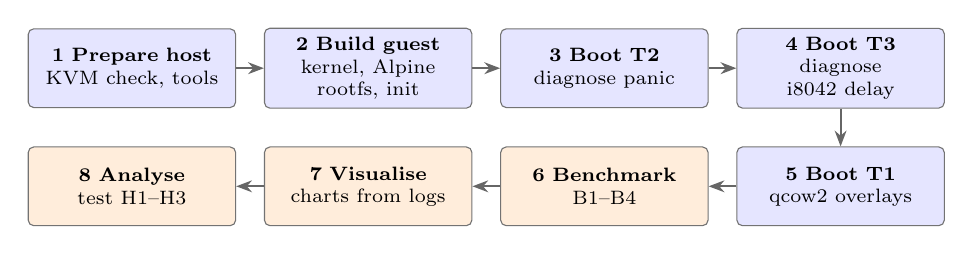
\begin{tikzpicture}[font=\scriptsize,
  st/.style={draw=black!55,rounded corners=2pt,fill=#1,minimum width=2.55cm,minimum height=1.0cm,align=center,text width=2.4cm},
  st/.default=blue!10,
  ar/.style={-{Stealth[length=2mm]},black!60,thick}]
\node[st] (s1) at (0,0) {\textbf{1 Prepare host}\\KVM check, tools};
\node[st] (s2) at (3.0,0) {\textbf{2 Build guest}\\kernel, Alpine rootfs, init};
\node[st] (s3) at (6.0,0) {\textbf{3 Boot T2}\\diagnose panic};
\node[st] (s4) at (9.0,0) {\textbf{4 Boot T3}\\diagnose i8042 delay};
\node[st] (s5) at (9.0,-1.5) {\textbf{5 Boot T1}\\qcow2 overlays};
\node[st=orange!14] (s6) at (6.0,-1.5) {\textbf{6 Benchmark}\\B1--B4};
\node[st=orange!14] (s7) at (3.0,-1.5) {\textbf{7 Visualise}\\charts from logs};
\node[st=orange!14] (s8) at (0,-1.5) {\textbf{8 Analyse}\\test H1--H3};
\draw[ar] (s1)--(s2); \draw[ar] (s2)--(s3); \draw[ar] (s3)--(s4); \draw[ar] (s4)--(s5);
\draw[ar] (s5)--(s6); \draw[ar] (s6)--(s7); \draw[ar] (s7)--(s8);
\end{tikzpicture}
\caption{Project workflow. Blue steps build and validate the four tiers; orange steps measure and analyse them.}\label{fig:workflow}
\end{figure}

%% =====================================================================
\section{Implementation and Experimental Setup}\label{sec:impl}

\subsection{Testbed}

All experiments ran on one desktop computer, described in Table~\ref{tab:testbed}. Before each benchmark the CPU frequency governor was set to \texttt{performance} so that frequency scaling did not add variance. Benchmarks ran inside a normal GNOME desktop session with background applications open but idle. The host passed \texttt{virt-host-validate} checks for hardware virtualization (VMX) and \texttt{/dev/kvm} access.

\begin{table}[ht]
\caption{Hardware and software of the testbed}\label{tab:testbed}
\footnotesize
\begin{tabular}{@{}ll@{}}
\toprule
Component & Version or specification \\
\midrule
CPU & Intel Core i5-7500, 4 cores, up to 3.8\,GHz, VT-x \\
Memory & 15.4\,GiB \\
Host operating system & Fedora 44 Workstation, Linux 7.2.13 \\
Hypervisor & KVM (\texttt{kvm}, \texttt{kvm\_intel} modules) \\
VMMs & QEMU 10.2.2; Firecracker 1.17.0 (static binary) \\
Container engine & Podman with \texttt{docker.io/library/alpine} \\
Benchmarking & hyperfine 1.20.0, \texttt{pidstat}, \texttt{ps}, \texttt{free} \\
MicroVM guest kernel & Linux 6.1.155, uncompressed ELF, Firecracker CI build \\
MicroVM root filesystem & Alpine 3.24.3 minirootfs in a 64\,MiB ext4 image, read-only \\
Traditional VM guest & Fedora 44 Cloud Base, Linux 6.19.10, qcow2 \\
\botrule
\end{tabular}
\end{table}

\subsection{Launch configurations}

The QEMU \texttt{microvm} tier (T2) is launched with
\begin{lstlisting}
qemu-system-x86_64 -M microvm,pit=off,pic=off -enable-kvm -cpu host -smp 1 -m 128 \
  -nodefaults -no-user-config -display none -serial stdio -no-reboot \
  -kernel vmlinux -append "console=ttyS0 root=/dev/vda ro init=/init reboot=t panic=-1 $ARGS" \
  -drive id=d,file=rootfs.ext4,format=raw,if=none,readonly=on -device virtio-blk-device,drive=d
\end{lstlisting}
where \texttt{-nodefaults} removes QEMU's default devices, \texttt{reboot=t} makes the guest reset through a triple fault, \texttt{-no-reboot} makes QEMU exit on that reset, and \texttt{panic=-1} turns a guest panic into an immediate reset rather than a hang. Firecracker (T3) is started with \texttt{firecracker --no-api --config-file} and a JSON configuration that specifies the same kernel, the same read-only root drive, one vCPU and 128\,MiB, and the boot arguments \texttt{console=ttyS0 reboot=k panic=-1 pci=off init=/init}. Firecracker adds the root device to the command line itself, and the guest requests a reset through Firecracker's minimal keyboard controller (\texttt{reboot=k}), on which Firecracker exits. Extra words passed to either launch script, such as \texttt{quiet}, \texttt{mode=dmesg} or the i8042 options, are appended to the kernel command line.

The traditional VM (T1) is launched with \texttt{-M q35 -enable-kvm -cpu host -smp 1 -m 1024 -snapshot -nic none -serial stdio -no-reboot}. The Fedora Cloud image expects a cloud provider to supply configuration at first boot through cloud-init; on a desktop no provider answers and boot would stall, so cloud-init was removed with \texttt{virt-customize}. T1 receives 1024\,MiB because Fedora does not boot reliably in 128\,MiB. The \texttt{-snapshot} option discards all disk writes when QEMU exits, so every T1 boot starts from an identical disk, and \texttt{-nic none} matches the microVMs, which have no network device.

The container tier (T4) runs \texttt{podman run --rm --network=none alpine true}.

\subsection{Copy-on-write images for the traditional VM}

The 620\,MB Fedora Cloud image is used as a read-only base. A 2.2\,MB \texttt{qcow2} overlay adds the boot-report service for benchmarking, and a separate 180\,MB overlay adds the \texttt{pciutils} package for interactive inspection. Neither overlay modifies the base, which would corrupt both overlays because they record differences from the base as it was when they were created.

\subsection{Configuration findings during implementation}\label{sec:findings}

Three problems appeared while building the microVM tiers. Each was diagnosed from kernel logs, and each is relevant to H2 because it concerns the virtual hardware rather than KVM.

\paragraph{Legacy timer hardware in QEMU microvm.}
The first T2 boot, without \texttt{pit=off,pic=off}, panicked 7.6\,ms into boot (Listing~\ref{lst:panic}). The kernel reported a divide error inside its console setup code, but the faulting instruction, marked \texttt{<65>} in the \texttt{Code:} line, is the start of a subtraction used for stack-protector checking, which cannot raise a divide error. On x86, exception vector 0 is the divide-error vector, and an external interrupt delivered on vector 0 is indistinguishable from one. QEMU's \texttt{microvm} machine type enables the legacy i8254 programmable interval timer (PIT) and i8259 programmable interrupt controller (PIC) by default when running on KVM~\cite{qemumicrovm}. We infer that the first PIT interrupt was delivered on vector 0 through a PIC that this kernel had not yet initialised. Disabling both devices removed the panic in every subsequent boot, and the kernel used the paravirtual KVM clock and the TSC deadline timer, both reported as available earlier in the same log. The \texttt{panic=-1} option worked as intended: the crashed VM exited after 0.248\,s instead of hanging.

\begin{lstlisting}[caption={Excerpt of the first T2 boot log (registers and call trace omitted)},label={lst:panic},float=ht]
[    0.007638] divide error: 0000 [#1] PREEMPT SMP PTI
[    0.007645] RIP: 0010:console_emit_next_record.constprop.0+0x1d4/0x2c0
[    0.007652] Code: ... 48 8b 45 d0 <65> 48 2b 04 25 28 00 00 00 0f 85 ...
[    0.007698] Kernel panic - not syncing: Attempted to kill the idle task!
real    0m0.248s
\end{lstlisting}

\paragraph{Keyboard controller probe in Firecracker.}\label{sec:i8042}
With the same guest, the first verbose Firecracker boot took 0.876\,s against 0.455\,s for QEMU \texttt{microvm}. Listing~\ref{lst:i8042} shows the cause: nothing was logged for 0.48\,s between two consecutive kernel messages, and the next message registered an AT keyboard on the \texttt{i8042} controller. Firecracker emulates a minimal i8042 so that the guest can request a reset through it~\cite{agache2020firecracker}; the guest's i8042 driver detects the controller and spends this time probing for devices behind it. QEMU \texttt{microvm} as configured here exposes no i8042, so T2 never pays this cost. Adding the four \texttt{i8042.*} kernel parameters listed earlier removed the delay without affecting the reset path.

\begin{lstlisting}[caption={Firecracker default boot: a 0.48\,s gap before the keyboard is registered},label={lst:i8042},float=ht]
[    0.258599] clk: Disabling unused clocks
[    0.742216] input: AT Raw Set 2 keyboard as /devices/platform/i8042/serio0/input/input0
[    0.747595] EXT4-fs (vda): recovery complete
\end{lstlisting}

\paragraph{Journal recovery on every boot.}
Listing~\ref{lst:i8042} also shows \texttt{EXT4-fs (vda): recovery complete}. Because the init script resets the VM without unmounting the root filesystem, the next boot replayed the ext4 journal, so each run's duration depended on the previous run. Attaching the root filesystem read-only in both VMMs removed this dependency; the guest never writes to disk, and a read-only image can also be shared safely by the 20 concurrent VMs in B4.

%% =====================================================================
\section{Results}\label{sec:results}

\subsection{Boot latency across tiers (B1)}

Table~\ref{tab:b1} and Fig.~\ref{fig:boot} report boot latency. All microVM runs used the \texttt{quiet} option and a read-only root filesystem. For T1 the table reports the time until the guest printed \texttt{BOOTED} over five runs, because one full T1 cycle takes about 15\,s; the full cycle including systemd shutdown averaged 15.25\,s (range 14.33--15.78\,s).

\begin{table}[ht]
\caption{Boot latency (B1). MicroVM and container figures are full boot-and-exit cycles after 3 warm-up runs; T1 is time until \texttt{BOOTED}}\label{tab:b1}
\footnotesize
\begin{tabular}{@{}lrrrrr@{}}
\toprule
Tier & Runs & Mean & Std.\ dev. & Min & Max \\
\midrule
T1 Traditional VM & 5 & 12.55\,s & 0.58\,s & 11.64\,s & 13.05\,s \\
T2 QEMU \texttt{microvm} & 30 & 162.5\,ms & 5.4\,ms & 155.0\,ms & 179.0\,ms \\
T3 Firecracker, default & 30 & 631.0\,ms & 3.4\,ms & 624.7\,ms & 637.9\,ms \\
T3 Firecracker, tuned & 30 & 118.6\,ms & 3.4\,ms & 113.9\,ms & 125.4\,ms \\
T4 Podman container & 30 & 135.4\,ms & 22.5\,ms & 113.7\,ms & 195.0\,ms \\
\botrule
\end{tabular}
\end{table}

\begin{figure}[ht]
\centering
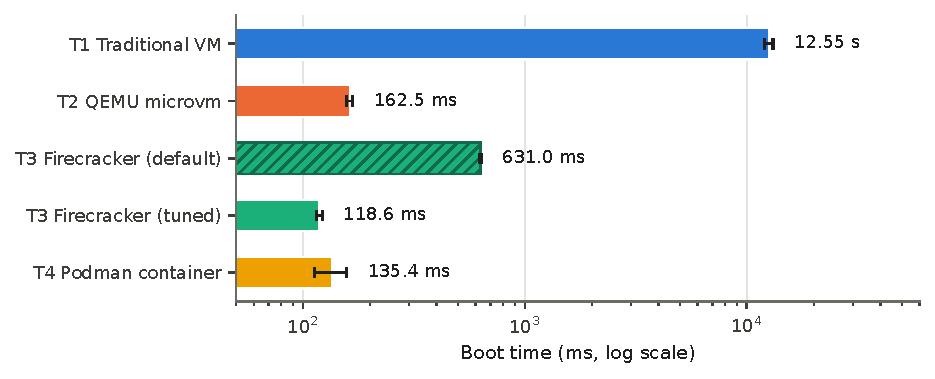
\includegraphics[width=\textwidth]{figures/fig_boot.pdf}
\caption{Mean boot latency of each tier on a logarithmic scale, with error bars showing one standard deviation. The hatched bar is Firecracker with its default boot arguments.}\label{fig:boot}
\end{figure}

The traditional VM was 106 times slower than tuned Firecracker and 77 times slower than QEMU \texttt{microvm}. These ratios are conservative, since the T1 figure stops at \texttt{BOOTED} while the microVM figures include the guest reset and the VMM's exit. All microVM configurations were highly repeatable, with standard deviations below 4\% of the mean. Tuned Firecracker was the fastest tier: 1.37 $\pm$ 0.06 times faster than QEMU \texttt{microvm} and 5.32 $\pm$ 0.16 times faster than Firecracker with default arguments, according to hyperfine's own comparison.

Tuned Firecracker also completed its cycle faster than Podman started and removed a container (1.14 $\pm$ 0.19 times faster). The container tier had by far the largest spread, from 113.7 to 195.0\,ms, so the two distributions overlap and the difference in means is small relative to the container's variability. The container figure also includes Podman's command-line tool and its \texttt{conmon} monitor, which are part of what a user experiences but are not intrinsic to containers. We therefore read this result as showing that a well-configured microVM is in the same start-up range as a container on this host, not that VMs are generally faster than containers.

\subsection{Guest kernel time versus VMM time (B2)}

Fig.~\ref{fig:breakdown} splits the mean microVM boot time into guest kernel time, measured from the guest log over 10 runs, and the remainder defined in Eq.~\eqref{eq:vmm}. The guest kernel reached \texttt{/init} after 42.5\,ms on QEMU \texttt{microvm} (standard deviation 1.7\,ms, range 39.9--45.7\,ms) and after 49.1\,ms on Firecracker (standard deviation 0.3\,ms, range 48.6--49.6\,ms). The VMM-side remainder was 120.0\,ms for QEMU and 69.5\,ms for Firecracker. By Eq.~\eqref{eq:red}, Firecracker reduces the VMM-side time by 42\%.

\begin{figure}[ht]
\centering
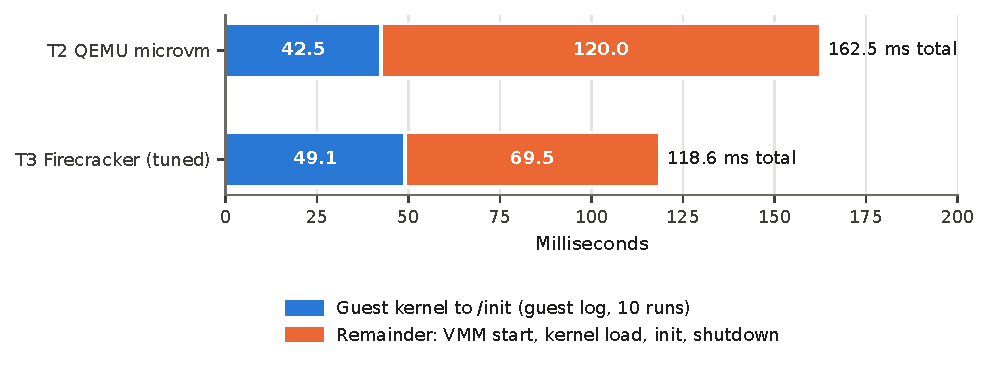
\includegraphics[width=\textwidth]{figures/fig_breakdown_microvm.pdf}
\caption{Mean boot time of the two microVMs split into guest kernel time (to \texttt{Run /init}) and the remainder: VMM start-up, VM creation and kernel loading, the init script, reset and VMM exit. Both boot the identical kernel and root filesystem.}\label{fig:breakdown}
\end{figure}

Two observations follow. First, with the guest held constant, almost the entire difference between the VMMs lies outside the guest kernel, which directly supports H2. Second, the guest kernel itself is 6.5\,ms slower on Firecracker. We did not trace the cause; plausible contributors are the remaining i8042 driver initialisation and the port I/O probes that Firecracker logs as unhandled (for example accesses to the PCI configuration ports \texttt{0xcf8} and \texttt{0xcfc}), each of which causes a VM exit. Firecracker's guest boot was also markedly more consistent, with a range of only 1\,ms across 10 runs against 5.8\,ms for QEMU, which is useful for platforms that must plan capacity around worst-case cold starts.

\subsection{Anatomy of a traditional VM boot}

Fig.~\ref{fig:t1} shows where the 12.55\,s of a T1 boot goes, averaged over five runs. About 2.41\,s elapse before the Linux kernel starts, covering QEMU start-up, SeaBIOS initialising the emulated PC and GRUB loading the kernel and initrd from disk. This pre-kernel phase alone is about 20 times longer than an entire tuned Firecracker cycle. The kernel then takes 1.20\,s, the initrd 3.50\,s to load drivers and locate the root disk, and systemd 5.44\,s to start services such as NetworkManager and sshd. The microVMs avoid the firmware, the bootloader and the initrd entirely, because the VMM loads the kernel directly and the disk driver is built into the kernel, and they replace systemd with a nine-line script. Inside the T1 guest, \texttt{lspci} listed the many emulated PCI devices of the \texttt{q35} machine, none of which exist in either microVM.

\begin{figure}[ht]
\centering
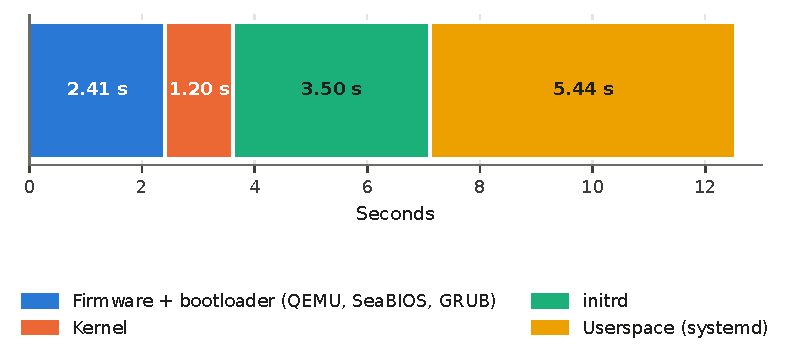
\includegraphics[width=\textwidth]{figures/fig_breakdown_t1.pdf}
\caption{Phases of the traditional VM boot (T1), mean of five runs. The firmware and bootloader phase is the host-measured time to \texttt{BOOTED} minus the total reported by \texttt{systemd-analyze}.}\label{fig:t1}
\end{figure}

\subsection{Cost of the serial console}

Table~\ref{tab:console} and Fig.~\ref{fig:console} compare boots that print the full kernel log to the emulated serial console with boots using the \texttt{quiet} option (20 runs each). Printing boot messages added 255.1\,ms to QEMU \texttt{microvm} and 222.9\,ms to Firecracker, increasing boot time by factors of 2.6 and 2.9. The console of a VM is an emulated 16550-style UART, and every character the kernel writes, as well as the status checks around it, is a port access that causes a VM exit to the VMM. A verbose boot writes thousands of characters. Firecracker's smaller penalty is consistent with a cheaper exit path, but both penalties exceed the entire quiet boot. For this reason all other microVM measurements in this paper use \texttt{quiet}, and the same consideration explains why production microVM platforms boot with the console disabled~\cite{fcspec}.

\begin{table}[ht]
\caption{Effect of a verbose serial console (20 runs each, mean $\pm$ standard deviation)}\label{tab:console}
\footnotesize
\begin{tabular}{@{}lrrr@{}}
\toprule
VMM & Verbose & \texttt{quiet} & Extra time \\
\midrule
T2 QEMU \texttt{microvm} & 415.1 $\pm$ 4.2\,ms & 160.0 $\pm$ 4.3\,ms & +255.1\,ms \\
T3 Firecracker, tuned & 342.3 $\pm$ 4.3\,ms & 119.4 $\pm$ 3.4\,ms & +222.9\,ms \\
\botrule
\end{tabular}
\end{table}

\begin{figure}[ht]
\centering
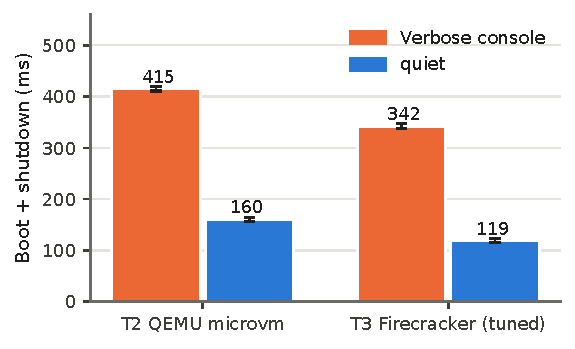
\includegraphics[width=0.62\textwidth]{figures/fig_console.pdf}
\caption{Boot-and-exit time with a verbose console and with \texttt{quiet}. Error bars show one standard deviation.}\label{fig:console}
\end{figure}

\subsection{Single-instance overhead (B3)}

Table~\ref{tab:b3} and Fig.~\ref{fig:memory} report the host resources used by one running instance, measured as the resident set size (RSS) of the VMM process, the physical memory it actually occupies. RSS includes guest memory that the guest has touched, since guest RAM is allocated inside the VMM process, so it is a measure of the total host cost of one idle instance rather than of the VMM alone.

\begin{table}[ht]
\caption{Host resources of one running instance (B3)}\label{tab:b3}
\footnotesize
\begin{tabularx}{\textwidth}{@{}lrrrY@{}}
\toprule
Tier & Guest RAM & Host RSS & Threads & VMM binary \\
\midrule
T1 Traditional VM & 1024\,MiB & 494.5\,MiB & 12 & 26\,MB, 78 shared libraries \\
T2 QEMU \texttt{microvm} & 128\,MiB & 113.8\,MiB & 4 & 26\,MB, 78 shared libraries \\
T3 Firecracker & 128\,MiB & 47.4\,MiB & 3 & 3.6\,MB, statically linked \\
T4 Container (process + \texttt{conmon}) & n/a & 2.4\,MiB & 1 + 1 & n/a \\
\botrule
\end{tabularx}
\end{table}

\begin{figure}[ht]
\centering
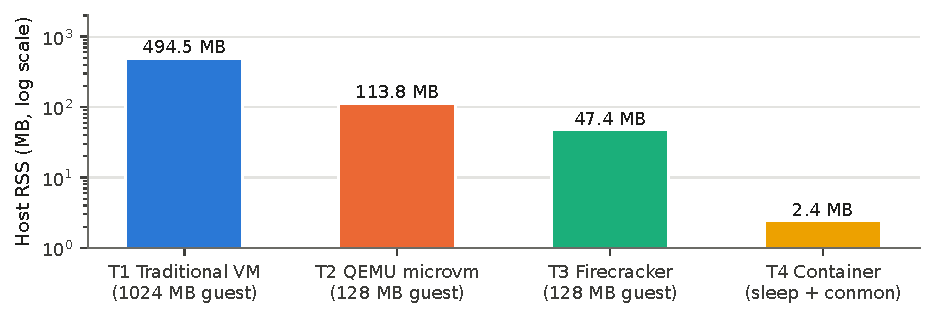
\includegraphics[width=\textwidth]{figures/fig_memory.pdf}
\caption{Host memory (RSS) of one running instance on a logarithmic scale. The container figure excludes the shared host kernel.}\label{fig:memory}
\end{figure}

For the same 128\,MiB guest, Firecracker used 58\% less host memory than QEMU \texttt{microvm} and one fewer thread. The binaries differ even more: QEMU is a 26\,MB executable that loads 78 shared libraries, whereas Firecracker is a single 3.6\,MB statically linked executable. Every library mapped into the VMM is code that runs with access to the guest's memory, so a smaller VMM also presents a smaller attack surface, which was an explicit design goal of Firecracker~\cite{agache2020firecracker}. The container is two orders of magnitude cheaper still, but only because it relies on the host kernel, which is precisely the shared component that weakens its isolation.

\subsection{Density and memory deduplication (B4)}

Table~\ref{tab:ksm} and Fig.~\ref{fig:ksm} report the results of starting 20 identical microVMs and then enabling KSM.

\begin{table}[ht]
\caption{Twenty concurrent microVMs with and without KSM (B4)}\label{tab:ksm}
\footnotesize
\begin{tabular}{@{}lrr@{}}
\toprule
Measurement & T2 QEMU \texttt{microvm} & T3 Firecracker \\
\midrule
Used memory, no VMs, $U_0$ (MiB) & 3346 & 3375 \\
Used memory, 20 VMs, $U_N$ (MiB) & 4746 & 4272 \\
Memory per VM, KSM off, Eq.~\eqref{eq:mvm} (MiB) & 70.0 & 44.9 \\
\texttt{pages\_shared} / \texttt{pages\_sharing} & 5113 / 134{,}649 & 0 / 0 \\
\texttt{general\_profit} $P$ (MiB) & 515.1 & 0 \\
Merged pages per VMM process (average) & 6988 (27.3\,MiB) & 0 \\
Memory per VM, KSM on, Eq.~\eqref{eq:mksm} (MiB) & 44.2 & 44.9 \\
\texttt{ksmd} CPU while scanning & 6.4\% & 0\% \\
\botrule
\end{tabular}
\end{table}

\begin{figure}[ht]
\centering
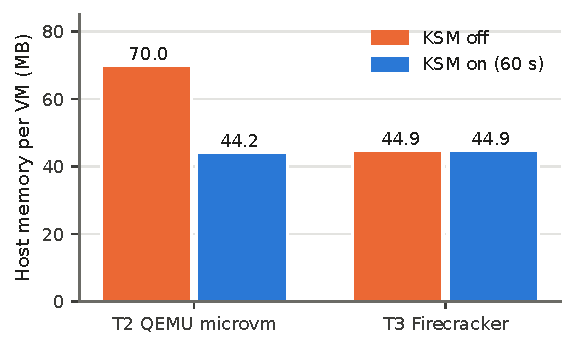
\includegraphics[width=0.62\textwidth]{figures/fig_ksm.pdf}
\caption{Host memory per VM with 20 identical microVMs, before and after 60\,s of KSM. KSM on is computed from the kernel's \texttt{general\_profit} counter.}\label{fig:ksm}
\end{figure}

For QEMU \texttt{microvm}, KSM saved 515.1\,MiB in total, reducing memory per VM by 37\% from 70.0 to 44.2\,MiB. Each merged page had on average $134{,}649/5113 \approx 26$ users. With only 20 VMs, this means that pages were duplicated within each VM as well as across VMs; a freshly booted, mostly idle guest contains many identical pages, most plausibly zero-filled ones. The per-process counter agrees with the global one: about 27.3\,MiB of each QEMU process was merged, close to the 25.8\,MiB per VM implied by $P/N$. Scanning cost the \texttt{ksmd} thread 6.4\% of one CPU.

For Firecracker, every KSM counter stayed at zero and \texttt{ksmd} used no CPU, although KSM was enabled system-wide in exactly the same way. KSM only scans memory that a process has marked as mergeable. QEMU marks guest memory as mergeable by default, whereas Firecracker does not, consistent with the Firecracker authors' recommendation to disable samepage merging as a side-channel mitigation~\cite{agache2020firecracker}. The most striking result of B4 is that Firecracker \emph{without} deduplication used about the same memory per VM (44.9\,MiB) as QEMU \texttt{microvm} \emph{with} deduplication (44.2\,MiB), without the scanning cost and without sharing pages between guests.

The second \texttt{free -m} reading after KSM showed a larger drop for QEMU (931\,MiB) than $P$ (515\,MiB). Because that reading covers the whole desktop over 60 seconds, we treat it as noisy and rely on the kernel's counters. Similarly, the sum of per-process RSS (2277\,MiB for 20 QEMU processes) exceeds $U_N - U_0$ (1400\,MiB), because RSS counts every shared page, including shared library pages, once in every process that maps it.

%% =====================================================================
\section{Discussion}\label{sec:discussion}

\subsection{Hypotheses}

Table~\ref{tab:verdict} summarises the evidence for each hypothesis.

\begin{table}[ht]
\caption{Hypotheses and evidence}\label{tab:verdict}
\footnotesize
\begin{tabularx}{\textwidth}{@{}lL{2.0cm}Y@{}}
\toprule
 & Verdict & Evidence \\
\midrule
H1 & Supported & MicroVMs reached a completed boot cycle 77 to 106 times faster than the traditional VM reached \texttt{BOOTED} (Table~\ref{tab:b1}). \\
H2 & Supported & With the guest held constant, VMM-side time was 42\% lower on Firecracker (Fig.~\ref{fig:breakdown}); one emulated legacy device cost 0.48\,s (Listing~\ref{lst:i8042}); legacy timer hardware decided whether the same kernel booted or panicked (Listing~\ref{lst:panic}); firmware and bootloader cost 2.41\,s in T1 (Fig.~\ref{fig:t1}). \\
H3 & Supported, with qualification & KSM saved 37\% per VM for QEMU at 6.4\% CPU (Table~\ref{tab:ksm}); Firecracker opts out by design and reached the same per-VM memory without deduplication. \\
\botrule
\end{tabularx}
\end{table}

Taken together, the results locate the cost of VM start-up in the virtual machine model and the software around the guest, not in hardware virtualization. All three VM tiers ran on the same KVM module, yet they differed by two orders of magnitude in start-up time and by an order of magnitude in memory. Within the microVMs, where the guest software was identical, the remaining differences were in the VMM process and in the devices it presented to the guest.

\subsection{Comparison with published results}

Our observations are consistent with published work, though the absolute numbers are not directly comparable because of different hardware, kernels and measurement endpoints. Agache et al.\ found QEMU about twice as slow as pre-configured Firecracker when booting to init with VMMs modified to exit on an I/O write~\cite{agache2020firecracker}. We measured unmodified VMMs over a full cycle that includes shutdown, and found QEMU \texttt{microvm} 1.37 times slower in total and 1.73 times slower in VMM-side time ($120.0/69.5$). The Firecracker specification targets 125\,ms or less from start to the guest's init with the serial console disabled and a minimal kernel and root filesystem~\cite{fcspec}; our complete tuned cycle, which includes init, reset and VMM exit, averaged 118.6\,ms on a 2017 desktop processor. For memory, Agache et al.\ reported VMM overheads of about 3\,MB for Firecracker and 131\,MB for QEMU, measured as non-shared memory excluding the binary and guest memory. Our RSS figures include touched guest memory, so they are higher for Firecracker and lower for QEMU, but they preserve the ordering. Li et al.\ reported about 8.76\,s for a QEMU/KVM VM to start~\cite{li2021lightweight}, the same order of magnitude as our 12.55\,s for a Fedora Cloud guest that additionally waits for systemd to report a fully started system.

Our container result resembles the argument of Manco et al.~\cite{manco2017lightvm} that a minimal VM can approach container start-up times. We reached that point with an unmodified Linux guest and a production VMM, but only after removing the i8042 probe; with default arguments Firecracker was 4.7 times slower than the container.

\subsection{Practical implications}

Three lessons apply beyond this testbed. First, configuration matters as much as the choice of VMM: a single default device probe erased Firecracker's advantage, and an emulated serial console more than doubled boot time for both VMMs. Benchmarks of microVMs should state their kernel command line. Second, the choice between microVMs and containers is primarily a trade-off between isolation and density rather than speed. In our measurements the start-up times were similar, but a container cost about 2.4\,MiB of extra host memory against about 45\,MiB for a microVM, while the microVM gave each workload its own kernel behind a hardware-enforced boundary. For untrusted, multi-tenant code the microVM is the safer choice; for trusted code, containers are denser. Approaches such as Kata Containers combine container tooling with VM isolation~\cite{katacontainers}. Third, memory deduplication can buy density, but a VMM designed for multi-tenant isolation can reach similar density by keeping its own footprint small, without sharing pages between tenants.

\subsection{Threats to validity}

\paragraph{Single host.} All measurements come from one desktop machine. Absolute numbers will differ on server hardware, other CPUs and other kernels, although the relative results are likely to hold because both microVMs share the same guest.

\paragraph{Desktop environment.} Benchmarks ran in a desktop session with background applications idle. The low standard deviations of the microVM measurements suggest that interference was small, but system-wide memory readings were affected, which is why B4 relies on KSM counters.

\paragraph{Minimal guest.} The microVM guest only prints a message and resets. A real function would add application start-up time, which this study does not measure.

\paragraph{Measurement endpoints.} T1 was measured to \texttt{BOOTED} over five runs, while the other tiers were measured over full cycles of 20 to 30 runs. The different endpoints make the T1 ratios conservative, and the small number of T1 runs widens its uncertainty.

\paragraph{Decomposition.} $T_{\mathrm{VMM}}$ contains a few milliseconds of guest activity after \texttt{/init} starts. This activity is the same in T2 and T3, so it does not affect their comparison, but $T_{\mathrm{VMM}}$ slightly overstates pure VMM time.

\paragraph{Different guest RAM sizes.} T1 used 1024\,MiB and the microVMs 128\,MiB, so the T1 memory figure reflects both its software stack and its larger allocation.

\paragraph{Causal attribution.} The explanation of the first kernel panic and of the 6.5\,ms guest difference are inferences from logs and from removing the suspected cause; we did not trace interrupts or VM exits directly.

%% =====================================================================
\section{Conclusion and Future Work}\label{sec:conclusion}

We compared a traditional VM, two microVMs and a container on one KVM host, holding the guest constant across the two microVM VMMs and splitting their boot time with two clocks. MicroVMs started 77 to 106 times faster than a traditional VM, because they remove what a traditional VM spends most of its time on: firmware, a bootloader, an initrd and a general-purpose service manager. With the guest held constant, Firecracker reduced VMM-side boot time by 42\% and single-instance host memory by 58\% compared with QEMU's \texttt{microvm}, and a tuned Firecracker microVM completed a boot cycle in about the same time as a Podman container start. Configuration details mattered greatly: legacy timer hardware caused a kernel panic, an emulated keyboard controller made default Firecracker 5.3 times slower, and a verbose console more than doubled boot time. Finally, KSM reduced QEMU microVM memory by 37\%, while Firecracker reached the same per-VM memory without deduplication.

Future work includes measuring snapshot restore, which avoids booting altogether~\cite{ustiugov2021reap,ao2022faasnap,lazarev2024sabre}; adding Cloud Hypervisor as a third VMM; running realistic function workloads inside the guest; tracing VM exits to explain the remaining guest-time difference; and repeating the study on server hardware with concurrent launches.

\backmatter

\bmhead{Acknowledgements}

We thank the faculty of the Department of Information Technology, Netaji Subhas University of Technology, for guidance in the Cloud Computing (ITITE503) course.

\section*{Declarations}

\begin{itemize}
\item \textbf{Funding:} Not applicable.
\item \textbf{Conflict of interest/Competing interests:} The authors declare no competing interests.
\item \textbf{Ethics approval and consent to participate:} Not applicable.
\item \textbf{Consent for publication:} Not applicable.
\item \textbf{Data availability:} All raw benchmark outputs (hyperfine JSON and Markdown exports, CSV files and text logs), terminal screenshots and generated figures are available at \url{https://github.com/xaidenwave/microvm-project}.
\item \textbf{Materials availability:} Not applicable.
\item \textbf{Code availability:} All launch and benchmark scripts, the guest init script, the systemd unit used for the traditional VM and the chart-generation script are available at \url{https://github.com/xaidenwave/microvm-project}. Large binary artefacts (guest kernel, root filesystem image, Fedora Cloud image and Firecracker binary) are not redistributed; the repository documents how to obtain or rebuild them.
\item \textbf{Author contribution:} All authors contributed to the design of the study, the experiments, the analysis and the writing of the manuscript. Sanyam Budwal led the project.
\end{itemize}

\bibliography{references}

\end{document}
